\documentclass[12pt]{article}

\usepackage{amsmath}
\usepackage[margin=0.75in]{geometry}
\usepackage[numbers]{natbib}
\usepackage{physics}
\usepackage[hyphens]{url}

\usepackage{fancyhdr}
\pagestyle{fancy}
\fancyhf{}
\rhead{Creative Destruction Lab}
\lhead{Week 1: Trapped ions}
\rfoot{Page \thepage}

\usepackage{graphicx}
\graphicspath{
	{images}
}

\usepackage[hidelinks]{hyperref}


\renewcommand{\phi}{\varphi}


\title{Week 1: Simulating quantum advantage with trapped ions}
\author{}
\date{}


\begin{document}

\maketitle

\thispagestyle{empty}


\section*{Introduction}

In 2019, the Martinis research group at Google ran an experiment on their Sycamore quantum computer, and they claimed it would take a classical supercomputer 10,000 years to simulate the same experiment~\cite{arute2019quantum}.
Thus, they concluded that this was the world's first example of quantum computational advantage: a quantum computer has drastically outperformed a classical one at a specific task, and the disparity will grow exponentially as the task is made more difficult.
Although different approaches have since been suggested to drastically improve on the classical bound of 10,000 years~\cite{pednault2019leveraging,pan2021simulating}, this remains a landmark feat of engineering on the road to general purpose quantum computation.

The task that was chosen for Google's demonstration is sampling from random circuits composed of 1- and 2-qubit gates.
While this sampling task was initially believed to provide no ``real-world'' applications, potential use cases are beginning to appear~\cite{aaronson2018certified}.
It's important to keep in mind that the current state-of-the-art gate-based quantum computers are limited by errors in the individual gates, which compound to produce unreliable results.
Indeed, the current generation of quantum computers is often referred to as ``noisy intermediate-scale quantum'' (NISQ) to emphasize their lack of error correction.
Using quantum computers for truly useful tasks (such as Shor's algorithm to factor integers out of reach of classical factoring techniques) is estimated to still be a long way into the future.

However, in a clever twist, Ref.~\citenum{arute2019quantum} actually takes advantage of the noisy nature of their quantum computer.
Their main result is the experimental determination of the linear cross-entropy benchmarking (XEB) fidelity~\cite{neill2018blueprint,boixo2018characterizing}:
\begin{align}
	\mathcal{F}_\mathrm{XEB}
	&= 2^N \langle P \rangle - 1
	= \frac{2^N}{S} \sum_{i=1}^S P(x_i) - 1,
\end{align}
where $N$ is the number of qubits, $P(x)$ is the exact probability of observing the bit-string $x$, and the average in angle brackets is performed over $S$ samples.
Ideally, $\mathcal{F}_\mathrm{XEB}$ should be 1, as would be the case if the samples $\{ x_i \}_{i=1}^S$ were drawn from the true distribution $P$; for example, if their quantum computer had no errors.
In practice, $\mathcal{F}_\mathrm{XEB} \ll 1$, due to imperfections in the realizations of the circuits.
Crucially, the authors were able to extrapolate $\mathcal{F}_\mathrm{XEB}$ based on their knowledge of the error rates of their quantum computer!

Superconducting qubits, such as those found in Sycamore are not the only possible foundation for a gate-based quantum computer.
Numerous other experimental implementations exist, but this week we will focus on ion trap quantum computers.
We can model 1-qubit gates as
\begin{align}
	R(\theta, \phi)
	&= \begin{pmatrix}
			\cos{\frac{\theta}{2}} & -i e^{-i \phi} \sin{\frac{\theta}{2}} \\
			-i e^{i \phi} \sin{\frac{\theta}{2}} & \cos{\frac{\theta}{2}} \\
		\end{pmatrix},
\end{align}
and 2-qubit gates as
\begin{align}
	M(\Theta)
	&= \begin{pmatrix}
			\cos{\Theta} & 0 & 0 & -i \sin{\Theta} \\
			0 & \cos{\Theta} & -i \sin{\Theta} & 0 \\
			0 & -i \sin{\Theta} & \cos{\Theta} & 0 \\
			-i \sin{\Theta} & 0 & 0 & \cos{\Theta} \\
		\end{pmatrix},
\end{align}
which can be combined in various ways to create circuits for an ion trap quantum computer~\cite{sorensen1999quantum,pogorelov2021compact}.

The tasks this week will involve applying these gates to a quantum state on a classical computer, with additional gates to simulate errors.
You will see how chaos can arise in individual measurements of random circuits, but also that it can be tamed by averaging over many measurements.


\section*{Suggested weekly tasks}

This section will guide you through several aspects of simulating an ion trap quantum computer using your classical computer.
The starting points provided for these tasks make use of Julia (\url{https://julialang.org/}), PastaQ (\url{https://github.com/GTorlai/PastaQ.jl/}), and ITensor (\url{https://itensor.github.io/ITensors.jl/v0.1/ITensorType.html}) but teams are encouraged to use the environments and libraries they prefer.


\subsection*{Task 1}

The output states of deep random circuits are chaotic, in the sense that slight perturbations in the circuits can lead to very different sampling probabilities.
Ref.~\citenum{arute2019quantum} makes an analogy between the visual patterns produced by a laser and samples produced by a quantum computer:
\begin{quote}
Owing to quantum interference, the probability distribution of the bitstrings resembles a speckled intensity pattern produced by light interference in laser scatter, such that some bitstrings are much more likely to occur than others.
\end{quote}
You will use this analogy to draw ``speckle patterns'' in order to visualize the states generated by perturbed random circuits.

The example script \texttt{run\_random\_circuit.jl} creates and runs a random circuit using the ion trap $R$ and $M$ gates, resulting in a random matrix product state (MPS), which represents a quantum state $\ket{\psi}$.
Extend this script to \textbf{extract the coefficients $\ip{x}{\psi}$ for each bit-string $x$ from the MPS}.
Please note that if you are using ITensor and PastaQ that PastaQ requires ITensor \texttt{v0.1.41}.
Unfortunately, there are functionalities in ITensor \texttt{v0.2.2} that would make this task very fast to complete, but they simply do not work in conjunction with PastaQ.
That being said, there are still many ways to do this Task!


The squared magnitude of each coefficient,
\begin{align}
	P(x)
	&= \abs{\ip{x}{\psi}}^2,
\end{align}
gives the probability of sampling the bit-string $x$ from $\ket{\psi}$.
\textbf{Plot the probability of each $x$ using a dot whose area is proportional to $P(x)$, like in Fig.~\ref{fig:speckle}, for several circuit widths and depths.}

\begin{figure}
	\centering
	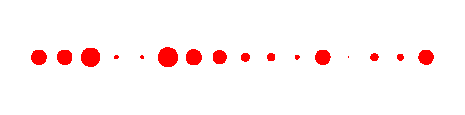
\includegraphics{images/speckle_N=004,depth=032}
	\caption{
		A ``speckle pattern'' displaying the probabilities of obtaining each of the 16 possible outcomes when sampling a 4-qubit state.
	}
	\label{fig:speckle}
\end{figure}

\medskip \noindent \textit{Bonus:}
Examine the change in the bond dimension of the generated MPS as the random circuits are made deeper.
Discuss the connection to entanglement entropy.


\subsection*{Task 2}

The outputs of sufficiently deep random circuits are very sensitive to slight perturbations in the circuit parameters, which can be seen by inserting errors.
For example, quantum computers are susceptible to bit-flip errors, modelled using
\begin{align}
	\sigma_x
	&= \begin{pmatrix}
			0 & 1 \\
			1 & 0 \\
		\end{pmatrix}.
\end{align}
Modify \texttt{run\_random\_circuit.jl} to \textbf{run one random circuit multiple times, but with a single bit-flip error at a random location in the circuit each time}.
The resulting speckle patterns should all be quite different; collect them into a collage.


\subsection*{Task 3}

As the depth of the random circuits is increased, the distribution of the probabilities $p = P(x)$ for a fixed output bit-string $x$ tends to the exponential distribution\footnote{
	In this context, it is sometimes referred to as the ``Porter--Thomas distribution''.
}:
\begin{align}
	p \sim 2^N e^{-2^N p},
\end{align}
where $N$ is the number of qubits.
For example, Fig.~\ref{fig:dists} shows that for random circuits on 8 qubits, those of depth 512 result in a cumulative distribution quite close to the expected one,
\begin{align}
	1 - e^{-2^N p},
\end{align}
while those of depth 1 do not.
\textbf{Demonstrate the convergence of the empirical cumulative distribution function of $p$ to the exact CDF of the exponential distribution with increasing circuit depth.}

\begin{figure}
	\centering
	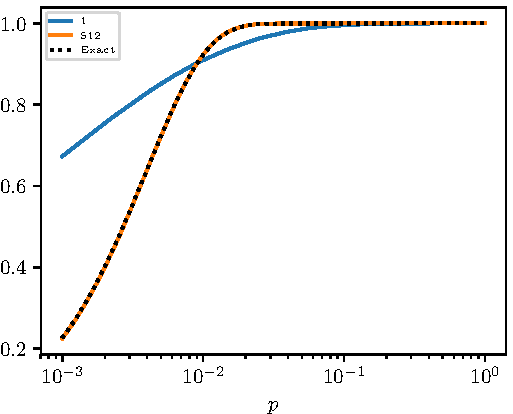
\includegraphics{images/dists_N=008}
	\caption{
		Empirical cumulative distribution functions of the probabilities $p$ for 8-qubit circuits of depth 1 and 512.
	}
	\label{fig:dists}
\end{figure}


\subsection*{Task 4}

One source of error in experimental realizations of quantum circuits is the inability to perfectly implement gates.
This could cause the observed distribution of $p$ to differ from the expected distribution, but visual comparison of entire distributions can be tedious and inexact.
A more quantitative approach to determine the difference between distributions is the linear XEB fidelity, $\mathcal{F}_\mathrm{XEB}$.
This is a single number that encodes the quality of the observed results.

Starting from a sufficiently deep random circuit, \textbf{perturb the angle of each 2-qubit gate by a fixed amount $\Delta \Theta$ to simulate a systematic error}.
Plot $\mathcal{F}_\mathrm{XEB}$ as a function of $\Delta \Theta$.


\subsection*{Business Application}

As apparent from your simulations, random circuits can be implemented on non-fault-tolerant NISQ hardware without error correction.
In the long term, people expect quantum computing to become feasible on universal, gate-based quantum computers with error correction, 
which would benefit many applications in industry.
Even with current NISQ hardware, methods exist to perform useful computations, such as the variational quantum eigensolver (VQE)~\cite{peruzzo2014variational},
which you will learn about in Week 3.
However, sampling from random circuits does not naively lend itself to such an obvious use case.
\textbf{Devise a potential business that could be built around sampling-based quantum computing with random circuits in the NISQ era.}
Integrate your idea into this week's \href{https://github.com/CDL-Quantum/CohortProject_2021/blob/main/Week1_Trapped_Ions/Business_Application.md}{Business Application}.

\section*{Additional Challenges}

The following optional tasks are of a broader scope, and might require additional research on your part.

\begin{enumerate}

\item Combine your speckle patterns from Task 2 into an animation that shows the changes in state probabilities as a single bit-flip error is moved around in a deep random circuit.

\item Download some samples and circuits from the data repository for Ref.~\citenum{arute2019quantum} at \url{https://datadryad.org/stash/dataset/doi:10.5061/dryad.k6t1rj8}.
Use these to reproduce $\mathcal{F}_\mathrm{XEB}$ values from the paper.

\item Run your quantum circuits on a trapped ion quantum computer, for example IonQ's quantum computers via Google Cloud Marketplace: \url{https://ionq.com/news/june-17-2021-ionq-quantum-computers-now-available-on-google-cloud/}.

\end{enumerate}

\bibliography{refs}
\bibliographystyle{unsrturl}

\end{document}
